%----------------------------------------------------------------------------------------
%	PACKAGES AND OTHER DOCUMENT CONFIGURATIONS
%----------------------------------------------------------------------------------------


\documentclass[12pt]{article} % Default font size is 12pt, it can be changed here

\usepackage{geometry}
\geometry{left=22mm,right=22mm, top=30mm, bottom=25mm}
\usepackage{setspace} 
\usepackage{hyperref}
\usepackage[ngerman]{cleveref}

\usepackage{color,soul}

\usepackage{subfigure}


\usepackage{eurosym}

\usepackage{hhline,float}

\usepackage{fancyhdr}

\usepackage{german}

\usepackage{pdflscape}
\usepackage[utf8]{inputenc}
\usepackage[T1]{fontenc}


\usepackage{longtable}
 
\usepackage{geometry} % Required to change the page size to A4
\geometry{a4paper} % Set the page size to be A4 as opposed to the default US Letter

\usepackage{graphicx} % Required for including pictures

\usepackage{booktabs}

\usepackage{float} % Allows putting an [H] in \begin{figure} to specify the exact location of the figure
\usepackage{wrapfig} % Allows in-line images such as the example fish picture



\linespread{1.2} % Line spacing

%\setlength\parindent{0pt} % Uncomment to remove all indentation from paragraphs

\graphicspath{{Pictures/}} % Specifies the directory where pictures are stored



\begin{document}
	
	\begin{titlepage}
		
		\newcommand{\HRule}{\rule{\linewidth}{0.5mm}} % Defines a new command for the horizontal lines, change thickness here
		
		\centering % Center everything on the page
		
		\begin{figure}[h] 
			\centering
			
\includegraphics[width=.4\textwidth]{Logo-FHNW}
		\end{figure}
		
		\textsc{\Large Dokumentation}\\[0.5cm] % Major heading such as course name
		\begin{doublespace}
			\HRule \\[1cm]
			{ \huge \bfseries Datenübertragung vom Pixhawk zum SBC}\\[1cm] % Title of your document
			\HRule \\[1cm]
		\end{doublespace}
		
		{\large \textbf{Auslesen der GPS-Daten vom Pixhawk über UART}}\\[1cm]

		{\large 17. Oktober 2016}\\[1cm] % Date, change the \today to a set date if you want to be precise
		
		{\large Saner Kevin}\\[1cm]
		{\large Institut für Automation}
		%\includegraphics{Logo}\\[1cm] % Include a department/university logo - this will require the graphicx package
		
		\vfill % Fill the rest of the page with whitespace
		
	\end{titlepage}
	
	\pagenumbering{arabic}
	\setcounter{page}{1}
	\pagestyle{fancy}
	\lfoot{18.10.2016} %left Foot
	\cfoot{\em Projekt FindMine} %Center Foot
	\rfoot{\thepage}
	
	\section{Einleitung}
	Das folgenden Beispiel zeigt auf welche Schritte durchgeführt werden müssen um die Verbindung zum Pixhawk herzustellen, sowie was unternommen werden muss damit die Kommunikation mit Hilfe des Mavlink Protokolls hergestellt werden kann. 

	\begin{description}
		\item[Voraussetzungen:]~\par
		\begin{itemize}
			\item Ubuntu Version 14.04 oder ähnlich
			\item QGroundControl unter Linux
			\item Pixhawk inkl. sämtlicher benötigter Peripherie
			\item 2 x FTDI-Kabel 3.3V
			\item Toolchain des Single Board Computer zum Cross-Kompilieren
		\end{itemize}
	\end{description}
	
	
	
	\section{QGroundControl}
	Um den Pixhawk in Betrieb zu nehmen muss auf dem Host-Computer ebenfalls die Applikation QGroundControl vorhanden sein. Die App kann als Imagedatei von \href{https://donlakeflyer.gitbooks.io/qgroundcontrol-user-guide/content/download\_and\_install.html}{QGroundControl} heruntergeladen werden, was dessen Installation relativ einfach macht. Die heruntergeladene Datei sollte nun an sicheren Ort kopiert werden. Anschliessend müssen noch die Benutzerrechte geändert werden.
	\\
	\noindent\hspace*{30mm} \textbf{Command:} \$ chmod +x ./QGroundControl.AppImage\\
	\\
	Dieser Befehl gibt dem momentanen Benutzer die Erlaubnis die Applikation auszuführen. Der folgende Befehl wiederum führt die Applikation schliesslich aus (oder doppelklicken).\\[0.2cm]
	
	\noindent\hspace*{30mm} \textbf{Command:} \$ ./QGroundControl.AppImage
	
	\section{Inbetriebnahme des Pixhawk}
	
	\subsection{Hardware}
	Bevor der Pixhawk ein erstes mal an der Computer angeschlossen werden kann, muss er zuerst entsprechend verkabelt werden. Denn einige Peripheriegerät sind zwingend notwendig für den Betrieb. Zur benötigten Peripherie gehören das GPS-Modul, der Taster sowie der Buzzer. Als Stromversorgung kann auch das mitgelieferte USB-Kabel verwendet werden, allerdings muss darauf geachtet werden, dass der verwendete USB-Port am Host-Computer die benötigte Spannung liefern kann. Für mehr Info: \href{https://3dr.com/wp-content/uploads/2014/03/pixhawk-manual-rev7.pdf}{QUICK START GUIDE}
	
	\begin{figure}[H]
		\centering
		\fbox{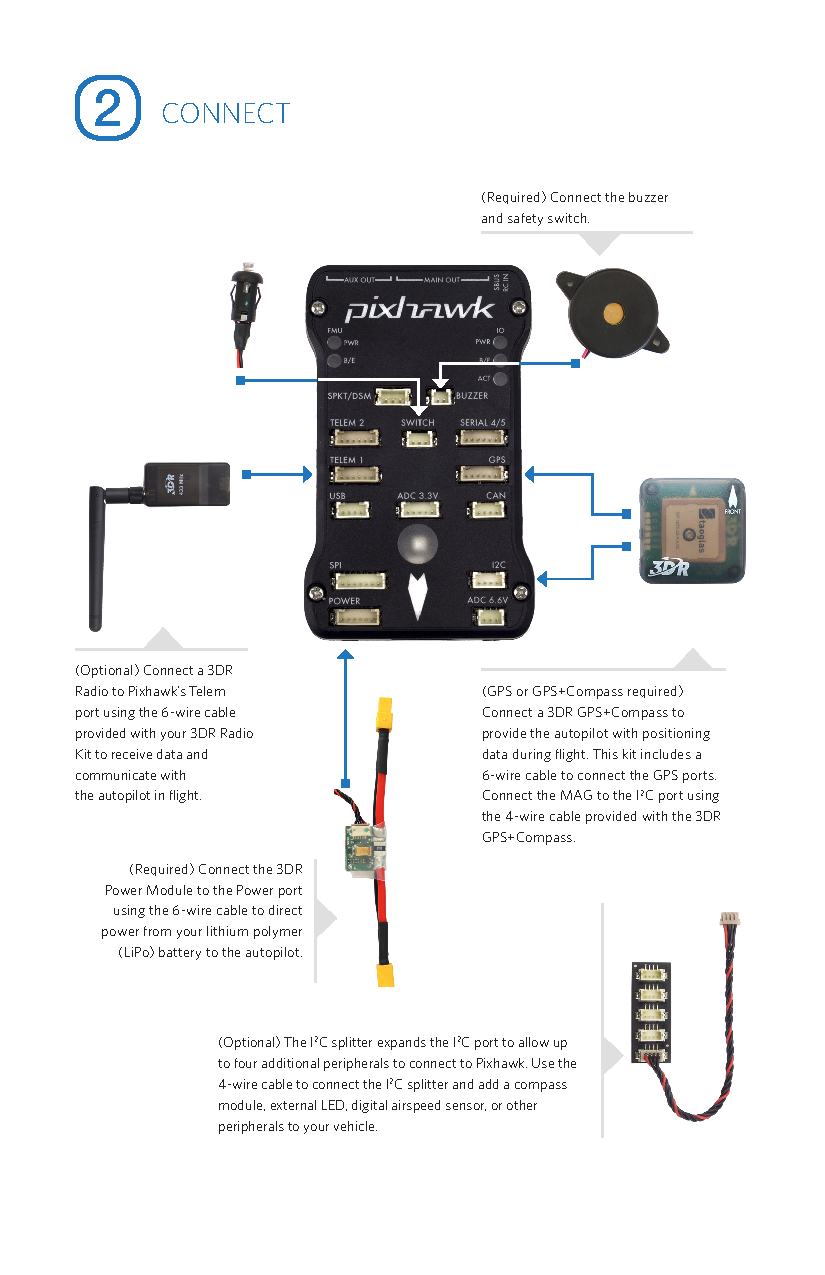
\includegraphics[scale=0.75]{connect}}
		\caption{Verkabelung des Pixhawk}
		\label{2}
	\end{figure}
	
	\subsection{Software}
	Der Pixhawk ist nun Betriebsbereit. Um nun die Sensoren zu kalibrieren wird empfohlen zuerst ein Firmwareupdate durchzuführen. Dabei wird auch die später benötigte Mavlink-Anwendung installiert. Es ist darauf zu achten, dass die PX4-Firmware und nicht die ArduPilot-Firmware geladen wird. Nachdem die Firmware erfolgreich installiert wurde, müssen die Sensoren kalibriert sowie auch der Airframe ausgewählt werden. 
	\\ \\
	QGroundControl führt dabei selbständig durch die Kalibration. Die Kalibration dient in erster Linie dazu die Maximalwerte der Beschleunigungssensoren zu bestimmen um die Lage des Pixhawk zu definieren.
	\\ \\
	Um schliesslich überprüfen zu können ob alle Systeme einwandfrei funktionieren empfiehlt es sich den Pixhawk unter freiem Himmel in Betrieb zu nehmen, denn nur so kann garantiert werden, dass GPS und Kompass exakte Daten liefern. War die Inbetriebnahme erfolgreich wird nun die aktuell Position des Pixhawks sowie die Ausrichtung in der QGroundControl-Applikation angezeigt, die Status-LED pulsiert dabei grün.
	
	
	\section{Mavlink}
	Um Daten auf den Pixhawk zu senden bzw. zu empfangen wird das Kommunikationsprotokoll Mavlink (Micro Air Vehicle Communication Protocol) verwendet. Mavlink streamt dabei die Daten über eine serielle Schnittstelle zu einer Kontrollstation. Als Kontrollstation kann zum Beispiel die vorher schon erwähnte Software QGroundControl dienen.
	\\Ziel der folgenden Arbeitsschritte ist es, die Mavlink-Messages mit einem C++-Programm interpretieren zu können. Diese Messages sollen dabei einerseits vom Host/Computer interpretiert werden können, in einem zweiten Arbeitsschritt soll das Programm aber für einen Phytec Single Board Computer kompiliert werden, damit dieser die Datenakquisition durchführen kann. Das verwendete C++-Programm basiert dabei grösstenteils auf dem UART-Beispiel auf \href{https://github.com/mavlink/c_uart_interface_example}{Github}.
	
	\subsection{Verkabelung}

	Um nun Daten vom Pixhawk auslesen zu können muss der Pixhawk zuerst entsprechend verkabelt werden. Erst durch diesen Schritt wird es möglich auf die Konsole des Pixhawk zuzugreifen. Wichtig ist dabei, dass ein 3.3V-FTDI-Kabel verwendet wird und kein 5V-FTDI-Kabel. Wahlweise kann der Pixhawk mit dem mitgelieferten USB-Kabel oder einer anderen Quelle mit Strom versorgt werden. Die Verkabelung muss nach folgendem Schema vorgenommen werden:
	
	\subsubsection{Verkabelung Konsole}
	
	Die Verkabelung der Konsole ist dabei nicht zwingend notwendig, kann aber hilfreich sein um sein um zu überprüfen ob das Mavlink-Protokoll auf dem verwendeten Port verfügbar ist. 
	\begin{description}
		\item
		\begin{tabular}{p{2cm}p{4cm}p{2cm}p{4cm}}
			\centering 
			\textbf{ Pixhawk} & \textbf{(Serial 4/5)} & \textbf{FTDI}& \\ \hline
			1 & +5V (red)	& 		& N/C				\\ \hline
			2 & S4 Tx	 	&		& N/C				\\ \hline
			3 & S4 Rx		&		& N/C				\\ \hline
			4 & S5 Tx		& 5		& FTDI RX (yellow)	\\ \hline
			5 & S5 Rx		& 4		& FTDI TX (orange)	\\ \hline
			6 & GND			& 1		& FTDI GND (black)	\\ \hline
			
		\end{tabular}
	\end{description}

	Im folgenden Bild wird dies auch noch grafisch dargestellt:

	\begin{figure}[H]
		\centering
		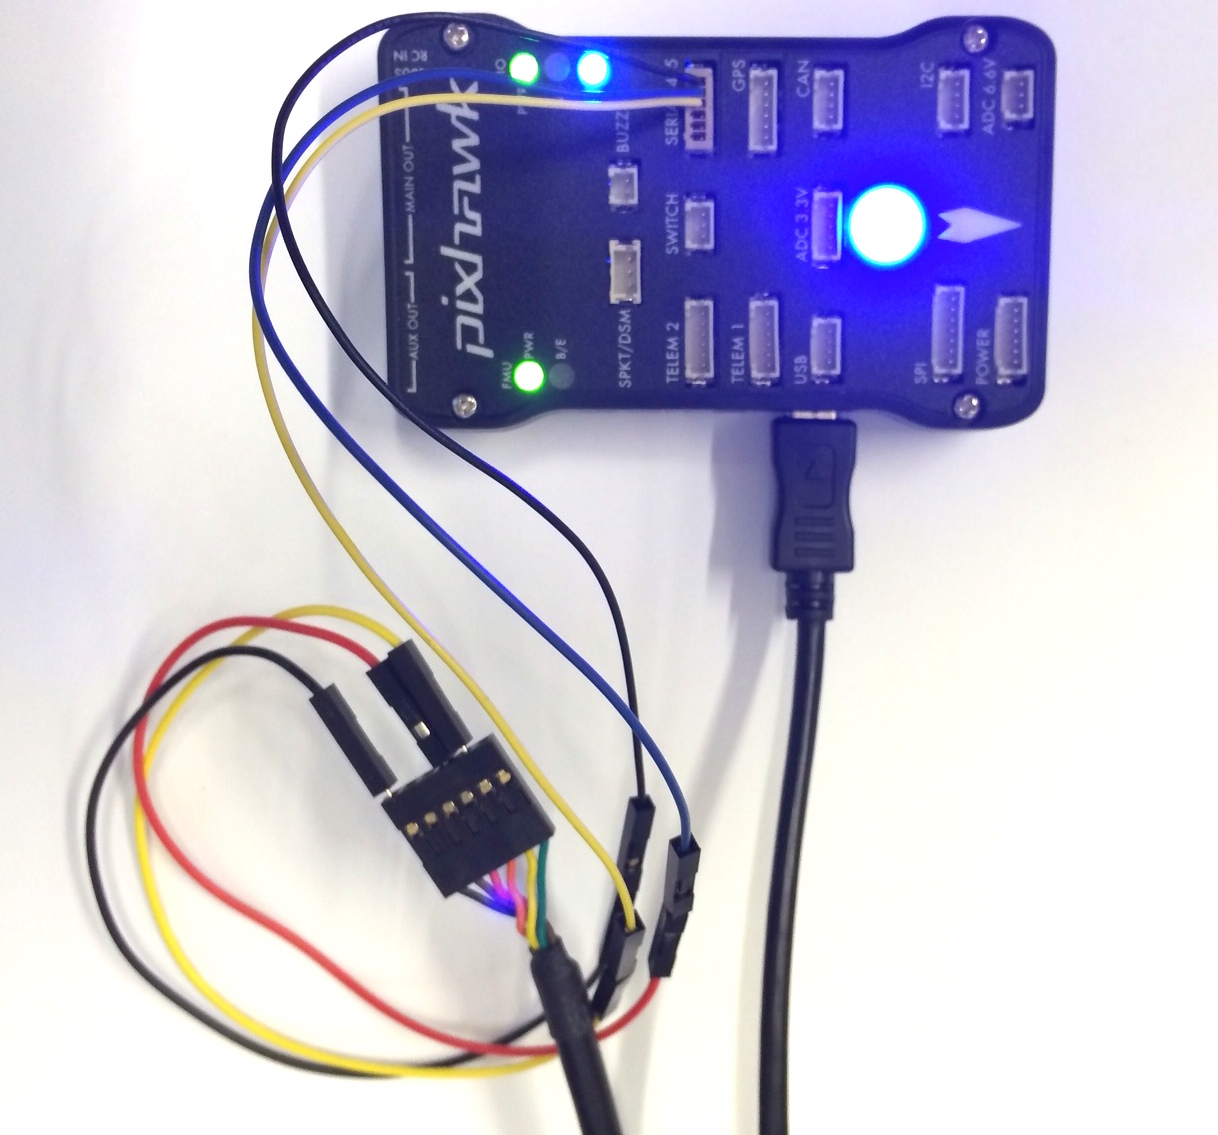
\includegraphics[scale=0.3]{Verkabelung_Mav}
		\caption{Verkabelung der Konsole}
		\label{2}
	\end{figure}

\subsubsection{Verkabelung Mavlink-Kanal}
	
	\noindent Um schliesslich Mavlink-Meldungen übertragen zu können, muss ein Port, auf welchem Mavlink-Meldungen gestreamt werden verkabelt werden. Die geeigneten Port sind Telem 1 und 2 sowie der USB-Port.	\\
	\textbf{TODO} Wie die Verkabelung mit SBC und Pixhawk schliesslich aussieht muss noch ausgearbeitet werden. Dabei ist zu beachten, dass die Datenübertragung über die UART-Ports des Pixhawk (Telem 1 und 2) nicht immer reibungslos zu funktionieren scheint, wohingegen die Übertragung über das USB-Kabel praktisch immer funktioniert.
	
	\begin{description}
		\item
		\begin{tabular}{p{2cm}p{4cm}p{2cm}p{4cm}}
			\centering 
			\textbf{ Pixhawk} & \textbf{Telem 1}& \textbf{FTDI}& \\ \hline
			1 & +5V (red)	& 		& N/C				\\ \hline
			2 & Tx (out)	& 5		& FTDI RX (yellow)				\\ \hline
			3 & Rx (in)		& 4		& FTDI TX (orange)				\\ \hline
			4 & CTS (in)	& 		& N/C	\\ \hline
			5 & RTS (out)	& 		& N/C	\\ \hline
			6 & GND			& 1		& FTDI GND (black)	\\ \hline
			
		\end{tabular}
	\end{description}
	
	Im folgenden Bild wird dies auch noch grafisch dargestellt:
	
	\begin{figure}[H]
		\centering
		\subfigure[]{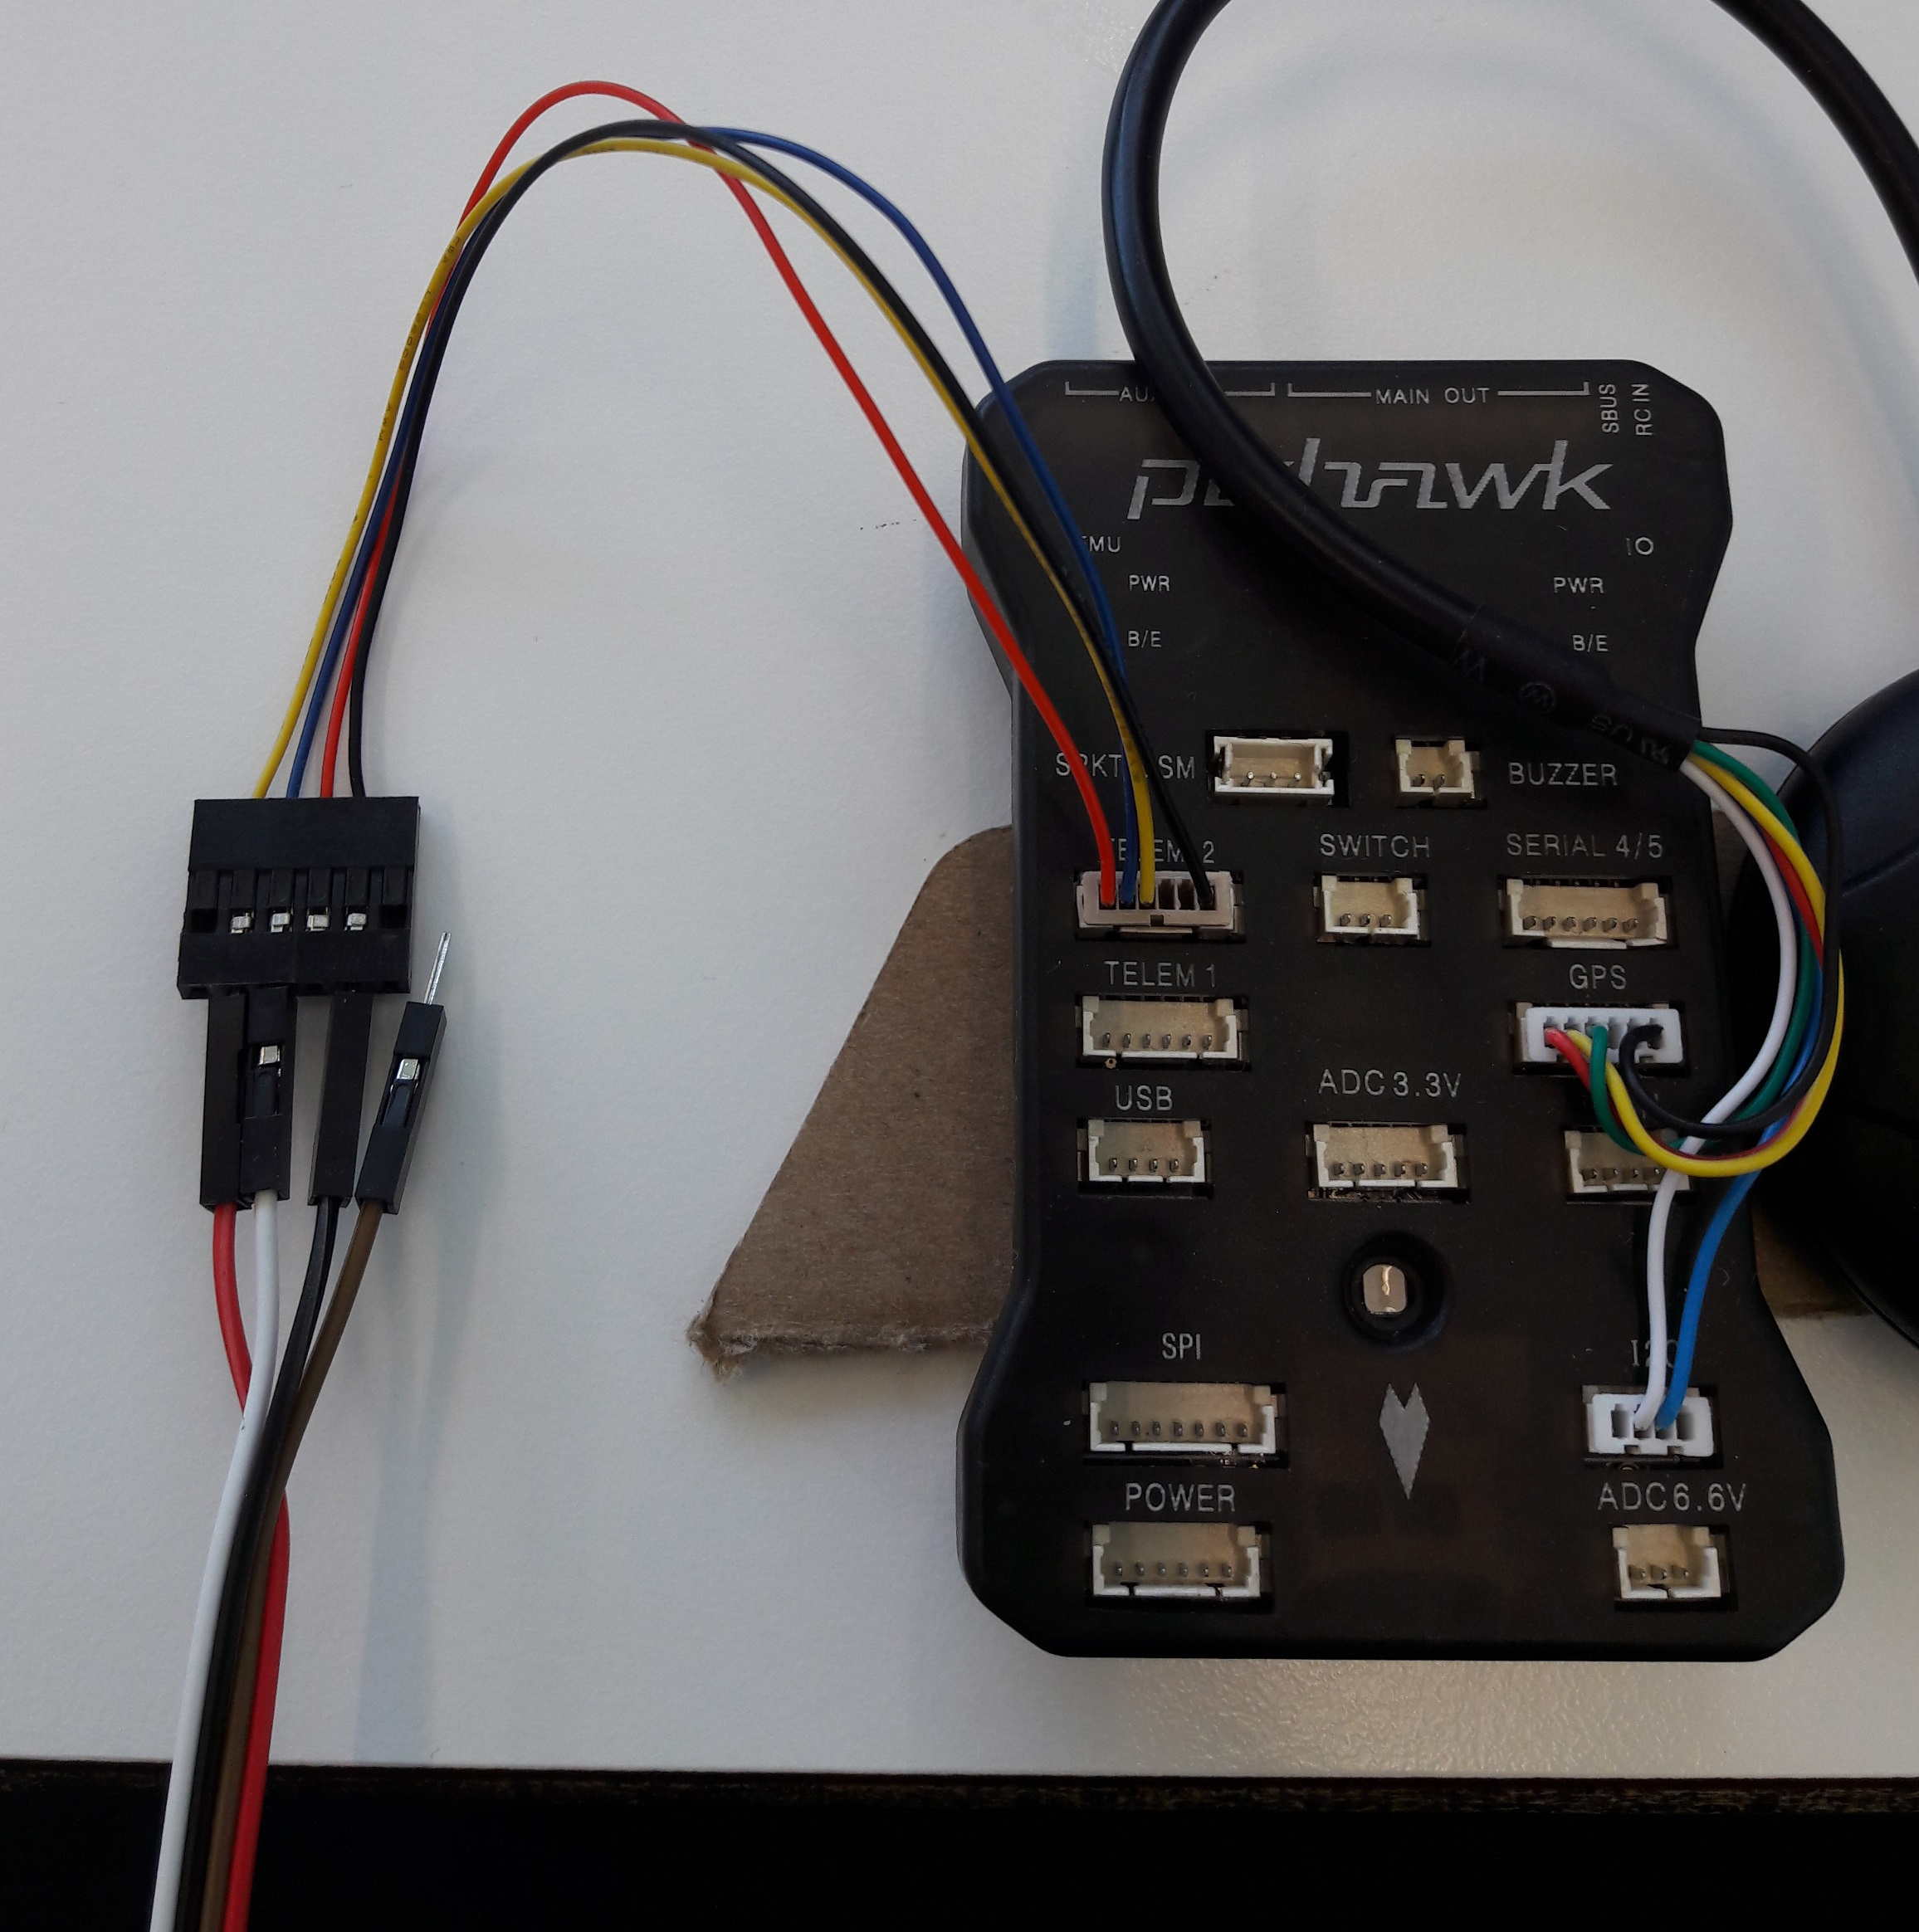
\includegraphics[scale=0.08]{PX_FTDI2}}\hfill
		\subfigure[]{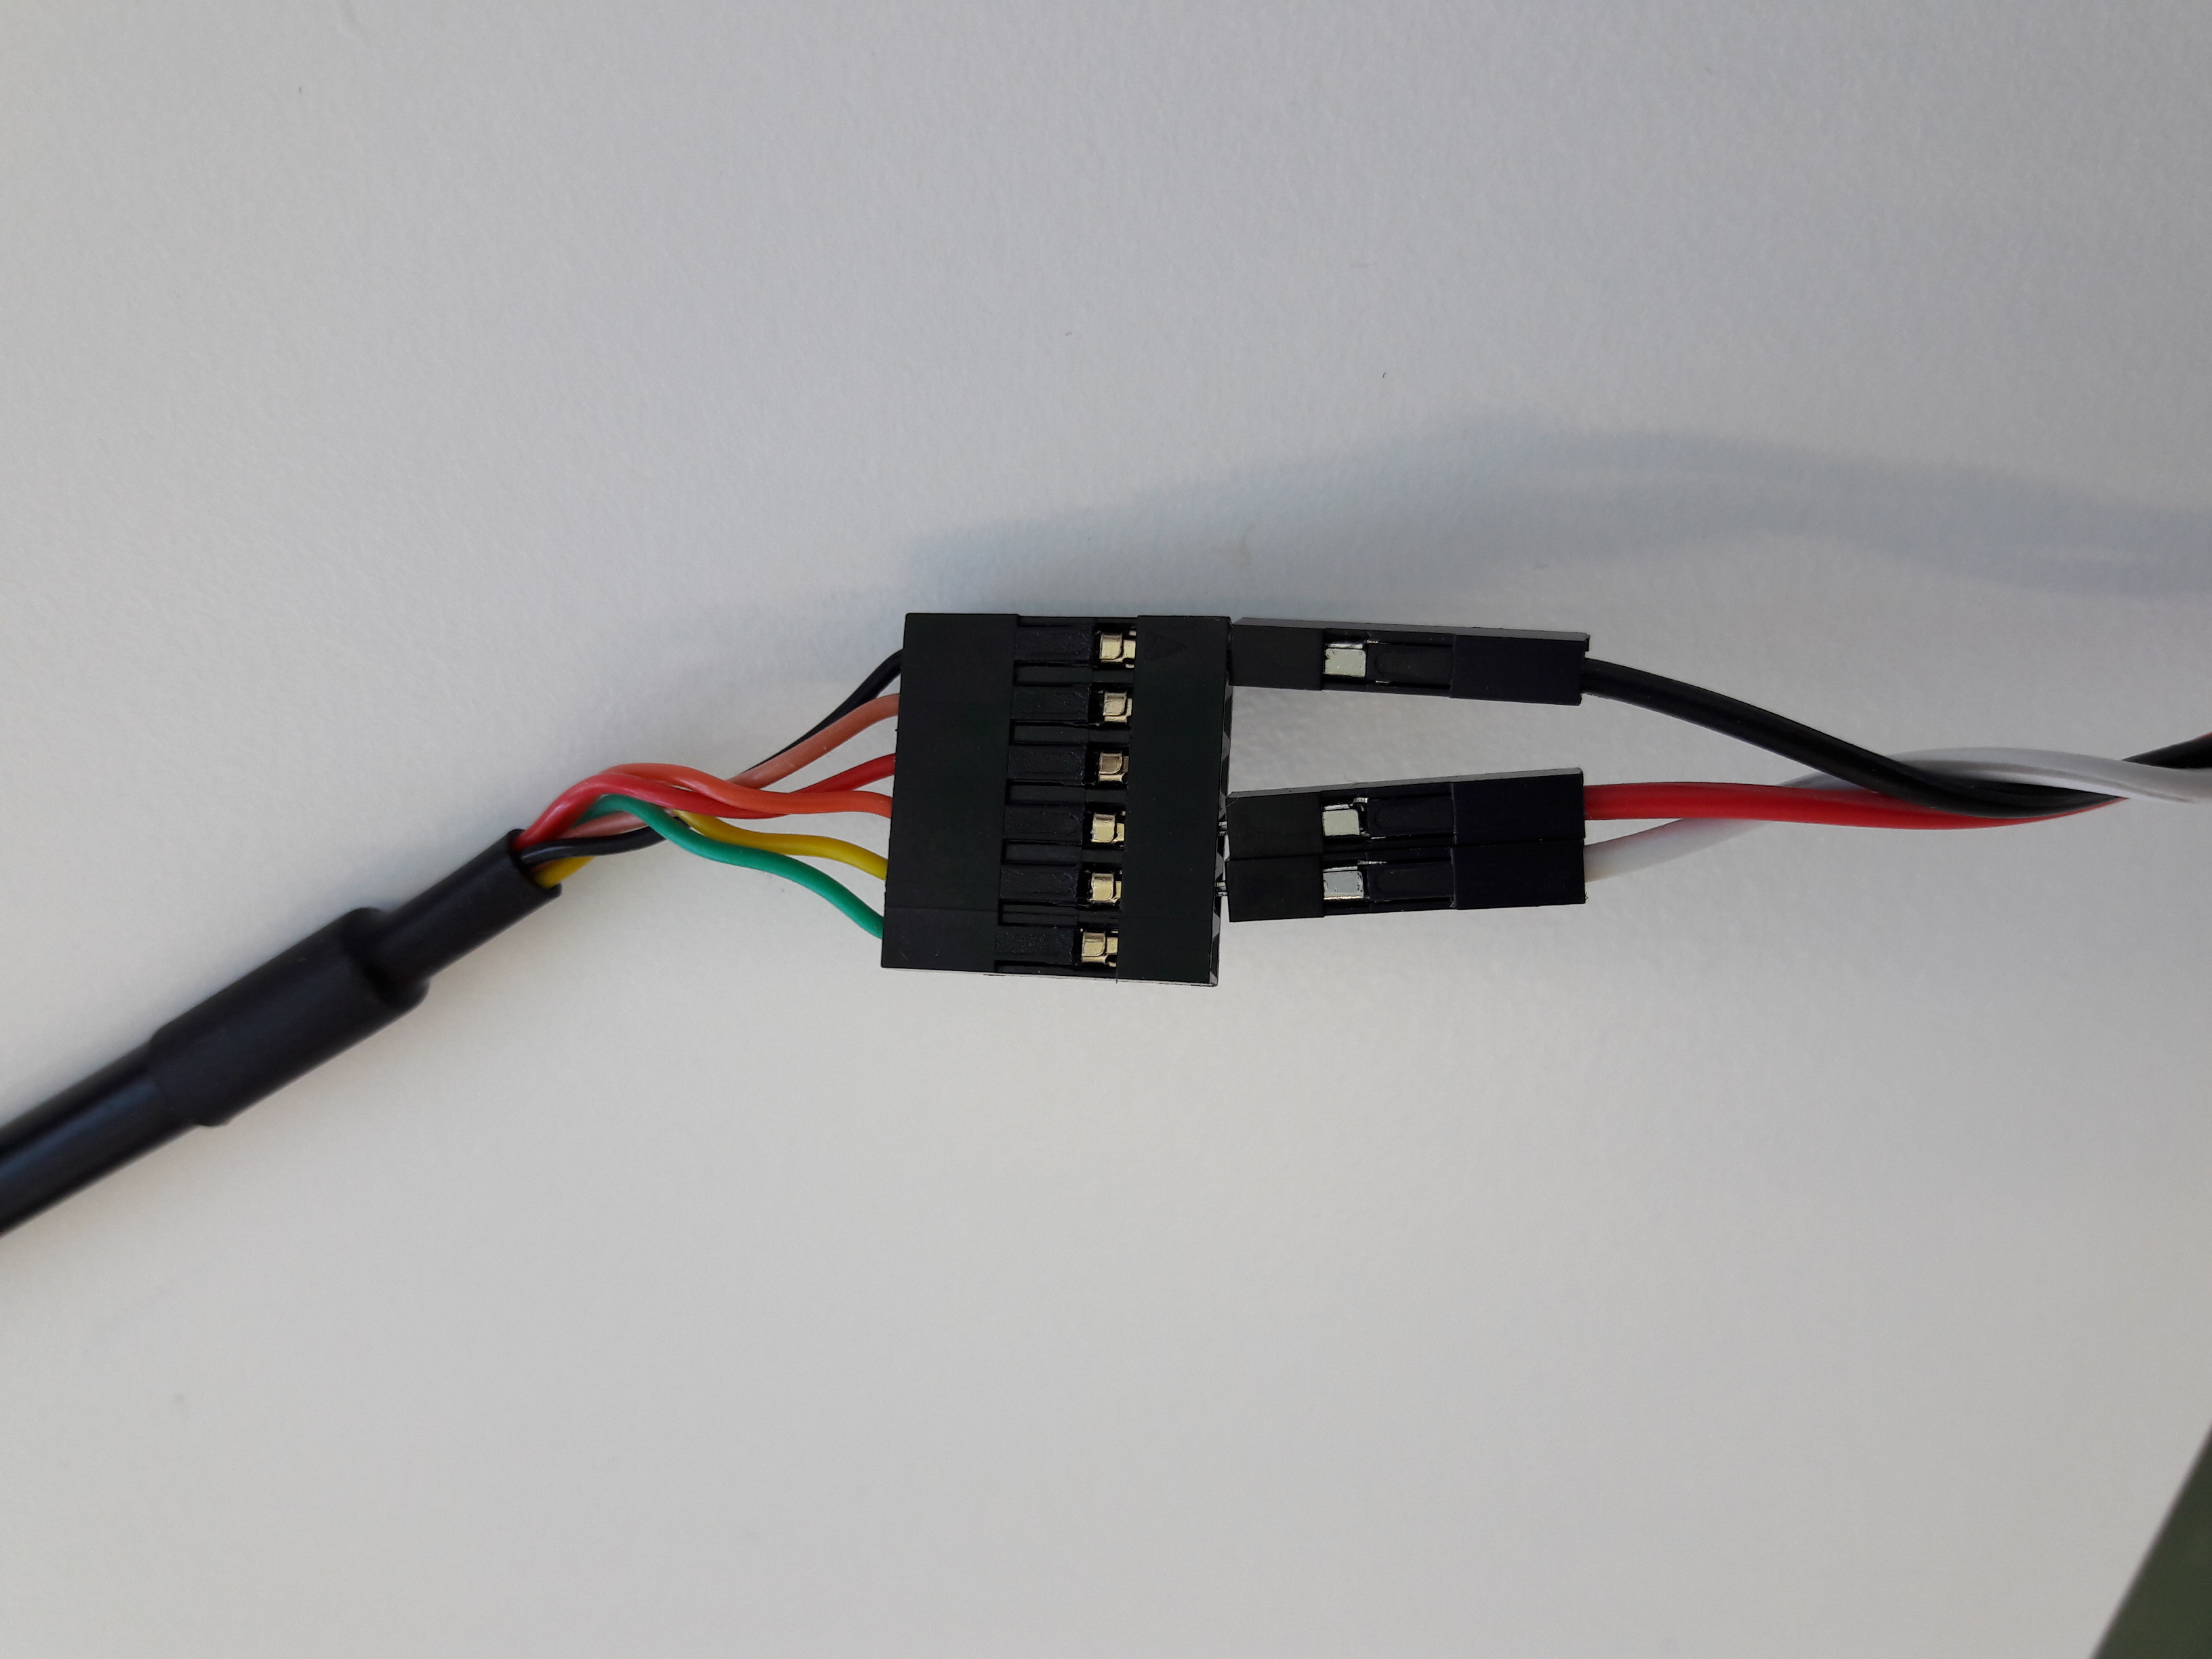
\includegraphics[scale=0.07]{PX_FTDI}}
		\caption{Verkabelung der Mavlink-Schnittstelle}
		\label{2}
	\end{figure}
	
	\noindent
	Kann der Telemetry-Port nicht verwendet werden, kann auch der serielle Port 4 verwendet werden. Dazu muss das FTDI-Kabel an die S4-Schnittstelle des Pixhawk angeschlossen werden (siehe Verkabelung Konsole). Diese könnte ausprobiert werden um die oben erwähnten Probleme mi der UART-Schnittstelle zu eliminieren. 
	\newpage
	\subsection{Setup} \label{Setup}
	
	Sind sämtliche Kabel angebracht entsteht das unten gezeigte Setup.
	\begin{figure}[H]
		\centering
		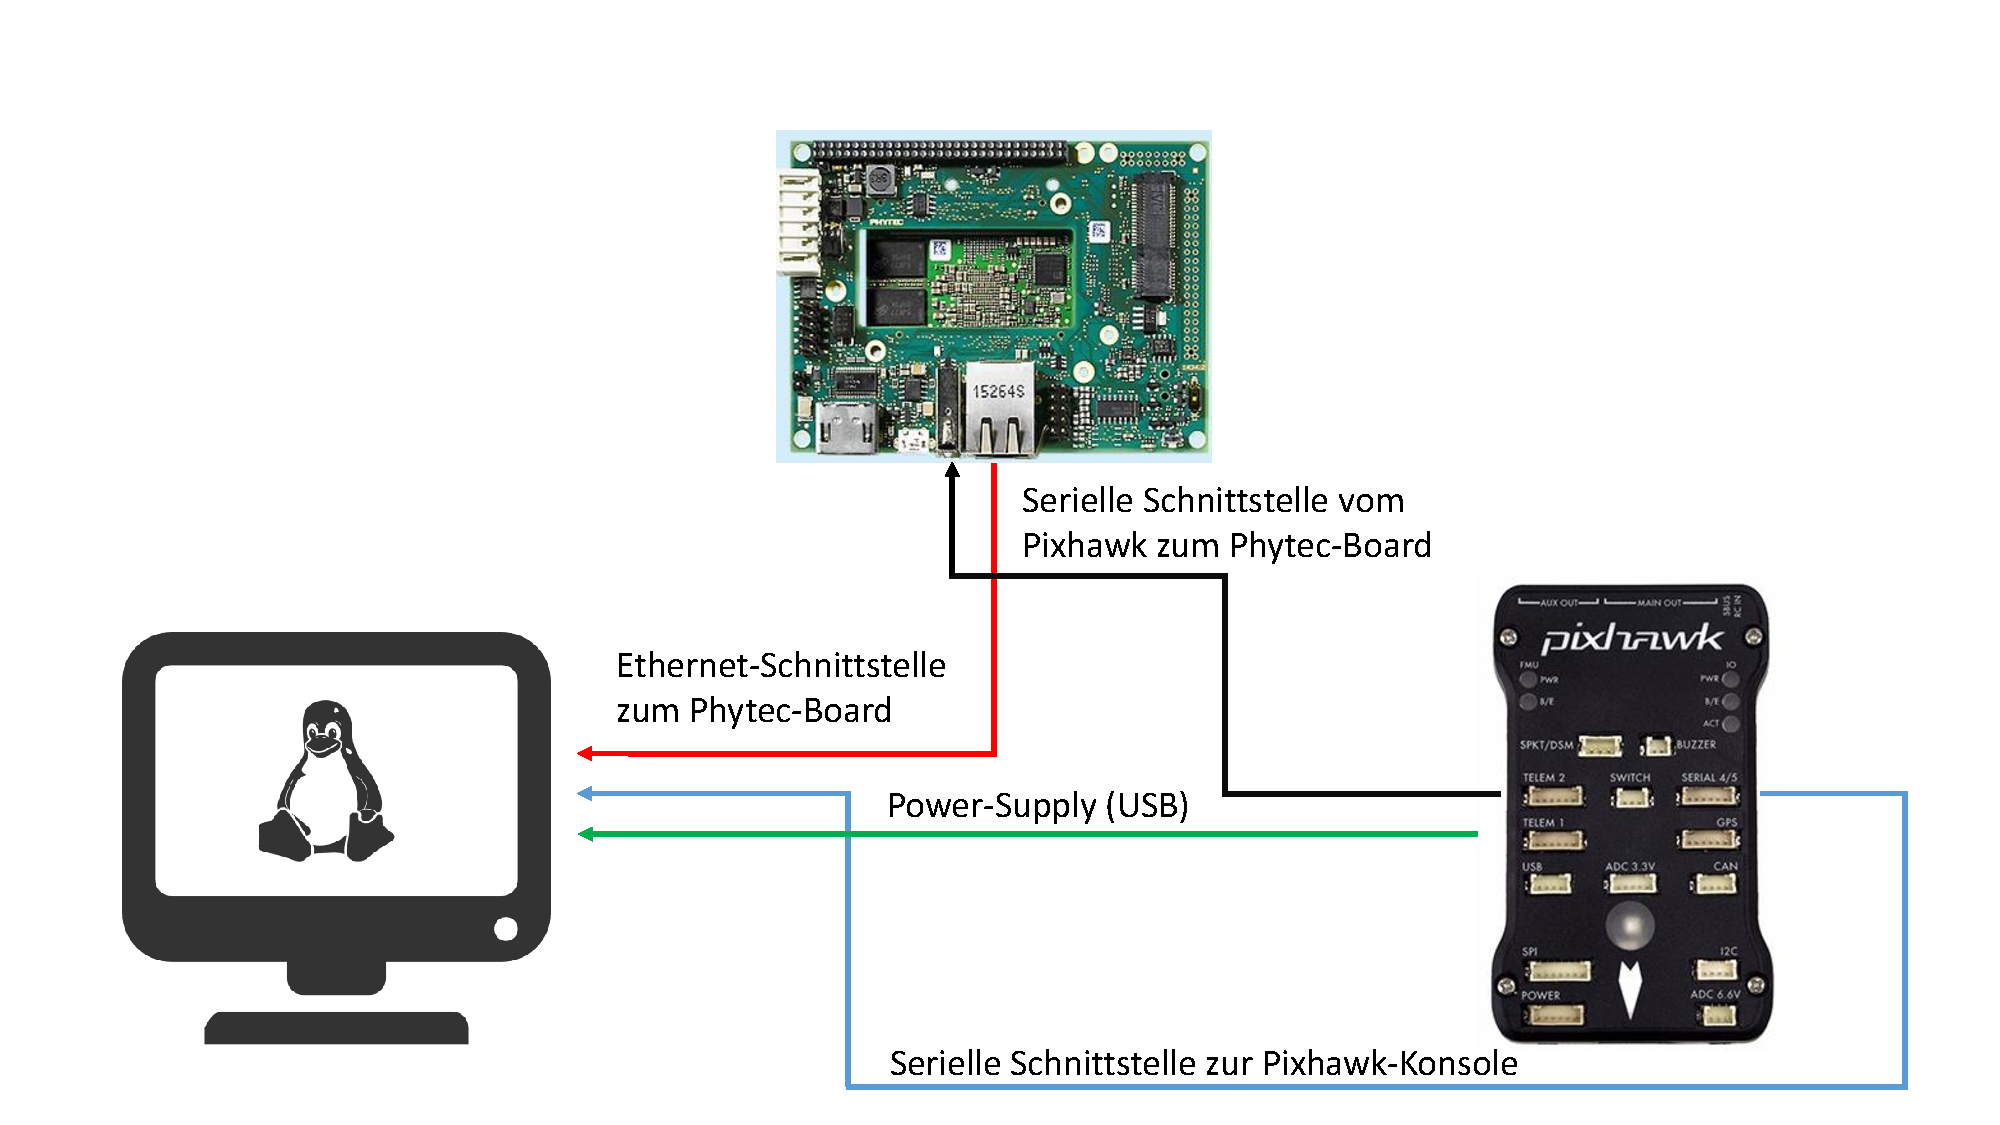
\includegraphics[scale=0.7]{Setup}
		\caption{Verkabelung des Pixhawk}
		\label{2}
	\end{figure}
	
	
	\subsubsection{Einloggen auf Pixhawk-Kosole}
	
	Der Anwender sollte nun in der Lage sein, sich auf die Konsole des Pixhawks einzuloggen. Dazu muss folgender Befehl eingetippt werden:
	\\[0.2cm]
	\noindent\hspace*{30mm} \textbf{Command:} \$ screen /dev/ttyUSB0 57600 8N1
	\\[0.2cm]
	Falls der Port-Name nicht gefunden wird, kann mit dem Befehl:
	\\[0.2cm]
	\noindent\hspace*{30mm} \textbf{Command:} \$ ls /dev/ttyUSB*
	\\[0.2cm]
	nach allen verfügbaren Ports gesucht werden. Der Anwender ist nun über die serielle Schnittstelle auf dem Pixhawk eingeloggt.\\
	\\
	Nun kann die Stromversorgung zum Pixhawk unterbrochen werden, damit dieser neu startet. Dabei werden unter anderen sämtliche Ports ausgegeben, auf welchen Mavlink empfangen werden kann. Ist der gewünschte Port nicht dabei, kann eine entsprechende Mavlink-Session über den jeweiligen Port wie folgt gestartet werden.
	\\[0.2cm]
	\noindent\hspace*{30mm} \textbf{Command:} \$ nsh> mavlink start -d /dev/ttyACM0
	\\[0.2cm]
	Über welche Ports eine aktive Mavlink-Session läuft ist von Bedeutung wenn versucht wird die gesendeten Daten entgegen zu nehmen und zu verarbeiten. Das folgende Beispiel zeigt einen Ausschnitt des Start-up-Prozederes des Pixhawks, daraus ist ersichtlich über welche Ports Mavlink-Messages gesendet bzw. empfangen werden.
	
		\begin{figure}[H]
			\centering
			\fbox{\includegraphics[trim = 22mm 240mm 30mm 22mm, clip, scale=0.75]{Mavlink_Out}}
			\caption{Programm Output}
			\label{2}
		\end{figure}
	
	\subsubsection{C++-UART-Mavlink-Schnittstelle}
	
	Wie schon erwähnt basiert das Programm auf dem UART-Interface-Beispiel verfügbar unter \href{https://github.com/mavlink/c_uart_interface_example}{GitHub}. Die entsprechenden Files können mit dem Befehl:
	\\[0.2cm]
	\noindent\hspace*{15mm} \textbf{Command:} \$ git clone https://github.com/mavlink/c\_uart\_interface\_example.git\\[0.2cm]
	\noindent
	auf dem Host-Computer kopiert werden. Die gesamten Definitionen des Mavlink-Protokoll können unter folgendem Link gefunden werden \href{https://pixhawk.ethz.ch/mavlink/}{Mavlink}. Da sind sämtliche Messages aufgeführt die vom Pixhawk gesendet werden können, und ebenso deren Definition.

	\paragraph{Programmablauf}\ \\
	Das Programm wurde dann noch mit ein paar Funktionen ergänzt, damit das Programm im FindMine-Projekt verwendet werden kann. Der Programmablauf sieht aktuell wie folgt aus: Zuerst versucht das Programm den ausgewählten Port zu initialisieren. Der Standard-Port ist dabei USB0 mit einer Baudrate von 57600. Um einen anderen Port zu verwenden können dem Programm Parameter übergeben werden, muss nicht extra der Code geändert werden. Nun wird versucht die System-IDs, des Pixhawk zu erfahren. Als nächstes wird vom Pixhawk eine Home-Position erwartet. Auf diese wird solange gewartet bis der Pixhawk ein GPS-Signal findet. Damit man das Programm auch ohne GPS-Log debuggen kann, kann dieser Schritt übersprungen werden. Allerdings erhält man so nur Dummy-Daten. Es ist zu beachten, dass das GPS-Signal nur empfangen wird wenn man sich unter freiem Himmel befindet.\\
	Als nächstes sendet der Host-Computer, eine Zielposition an den Pixhawk, die dieser dann zu erreichen versucht. Diese Funktion (enable/disable offboard control) wird wahrscheinlich zu einen später Zeitpunkt nicht mehr verwendet und kann entfernt werden.\\
	Nun versucht der Host-PC Daten vom Pixhawk zu lesen. Da das Lesen der Daten, insbesondere der Positionsdaten, die Hauptaufgabe des Programms ist wird dies nun in einer Endlosschlaufe ausgeführt. Der Main-Loop wird momentan maximal im Sekundentakt, also mit 1 Hz ausgeführt. Diese Frequenz muss noch optimiert werden. Der Pixhawk liefert die Daten mit einer Maximalfrequenz von 10 Hz, dies ist also das Maximum, dass erreicht werden kann. Dabei werden ähnlich dem SBGC-Interface, die Daten in ein CSV-File geschrieben. Die Positionsdaten, können dabei als relative wie auch als globale Werte empfangen werden. Die Positionsdaten werden zudem mit dem Zeitstempel des Pixhawk wie auch des SBCs ergänzt. Der Zeitstempel des Pixhawk entspricht dabei i.d.R. der seit Systemstart vergangenen Zeit in Mikrosekunden (siehe \href{https://pixhawk.ethz.ch/mavlink/#HIGHRES_IMU}{HIGHRES\_IMU}). Die Art wie der Zeitstempel des Pixhawk kreiert wird entspricht der des SBGC-Interface.\\
	Zur Zeit werden auch noch die restlichen Daten die vom Pixhawk gesendet werden in ein File abgespeichert. Dies geschieht bei jedem 50 Durchlauf des Main-Loop. Stellt sich heraus, dass diese Daten ebenfalls nie verwendet werden, kann dieser Programmteil ebenfalls entfernt werden.
	
	\paragraph{Kompilation}\ \\
	Das Programm kann unter Ubuntu mit den im Projekt enthaltenen Make-Files problemlos kompiliert werden. Um das Programm für den SBC kompilieren zu können, müssen die Anweisungen im Cross-Compilation-Guide befolgt werden.\\ \\\
	\noindent
	Um das eben erstellte Programm zu starten muss der folgende Befehl ausgeführt werden:
	\\[0.2cm]
	\noindent\hspace*{30mm} \textbf{Command:} \$ ./mavlink\_control -d /dev/ttyACM0\\ \label{Exec Mav}
	
	\subsubsection{Ergebnis}
	Damit das Programm nun auf dem Phytec SBC ausgeführt werden kann, muss das entsprechende Setup erstellt werden (siehe \ref{Setup}). Zudem muss der entsprechende Port ausgewählt werden, ist der Port nicht verfügbar bricht das Programm mit einer Exception ab. Ist alles korrekt konfiguriert können der Pixhawk und der Phytec SBC nun über Mavlink kommunizieren, dass heisst es können Kommandos gesendet wie auch empfangen werden.\\
	\\
	Das Programm kann mit demselben Befehl wie beim Starten vom Host-Computer ausgeführt werden (siehe \pageref{Exec Mav}). Unter der Bedingung, dass der Pixhawk ebenfalls korrekt initialisiert und über GPS-Signal verfügt, wird nun ein File mit den erhaltenen GPS-Daten sowie den IMU-Daten erstellt, dass in das Post-Processing miteinbezogen werden kann.
	

\newpage
\renewcommand\refname{Literaturverzeichnis}
\begin{thebibliography}{99} % Bibliography - this is intentionally simple in this template
	\raggedright
	
	\bibitem{1}
	Pixhawk Autopilot:
	\newblock {\em Quick Start Guide}
	\newblock [online] Available at: https://3dr.com/wp-content/uploads/2014/03/pixhawk-manual-rev7.pdf [Zugriff am 28.02.2017]
	
	\bibitem{2}
	Lorenz Meier:
	\newblock {\em C-UART Interface Example}
	\newblock [online] Available at: https://github.com/mavlink/c\_uart\_interface\_example [Zugriff am 28.02.2017]
	
	\bibitem{3}
	ETHZ:
	\newblock {\em Mavlink Common Messages Set}
	\newblock [online] Available at: https://pixhawk.ethz.ch/mavlink/e [Zugriff am 28.02.2017]



\end{thebibliography}

	
\end{document}